
%(BEGIN_QUESTION)
% Copyright 2010, Tony R. Kuphaldt, released under the Creative Commons Attribution License (v 1.0)
% This means you may do almost anything with this work of mine, so long as you give me proper credit

Two instrument technicians are arguing over the stability of a PID control system.  The process variable is oscillating around setpoint like this:

$$\includegraphics[width=15.5cm]{i04732x01.eps}$$

One technician says the gain of the PID controller is set at too high a value.  The other technician says this oscillation is the result of integral (reset) action being too aggressive.  What do you think?  Do you agree with one of these technicians more than the other?  If so, why?

\underbar{file i04732}
%(END_QUESTION)





%(BEGIN_ANSWER)

Either too high of gain or too aggressive reset may cause oscillation to occur.  The cause can also be completely external to the controller as well (e.g. excessive damping in the transmitter).

\vskip 10pt

I recommend awarding half credit for agreeing with the first technician (gain too high), half credit for agreeing with the second technician (reset too aggressive), and full credit if the student says either could be true.  Full credit should be given if the student recognizes potential external causes not limited to excessive P or I.

%(END_ANSWER)





%(BEGIN_NOTES)

{\bf This question is intended for exams only and not worksheets!}

%(END_NOTES)


